\subsection{Electric and weighting fields}
\label{subsec:efield_wfield}
The radial component of the electric field of a true coaxial germanium crystal can be calculated analytically 
\begin{equation}
  \label{eq:EFieldAnalytical}
  |E(r)| = \frac{eN_{A}}{2\epsilon_{0}\epsilon_{R}} r + \frac{V - (eN_{A}/4\epsilon_{0}\epsilon{R})(r_{2}^{2}-r_{1}^{2})}{r \ln(r_{2}/r_{1})},
\end{equation}
with inner and outer radii $r_1$ and $r_2$ and $V = \varphi(r_2) - \varphi(r_1)$. The other components $E(\varphi,z)$ could be calculated analytically, but they are zero.
The weighting potential and field of the segments cannot be calculated analytically, but the numerical method to calculated the electric field and the weighting fields are the same. By comparing the results of the numerical calculation of the electric field and the analytical one, one gains trust into the calculation of the weighting fields.


The result of the analytic and numeric calculation of the electric field for a 18 fold segmented true coaxial n-type germanium detector are shown in \figref{fig:efields}. The simulated detector has a inner radius of $r_{1} = 0.005$~m and an outer radius $r_{2} = 0.0375$~m. The height is $0.07$~m. The simulated applied voltage is $3000$~V on the core. The charge carrier density is $0.68\cdot 10^{10} \text{~cm}^{-3}$, which corresponds to a depletion voltage of $2500$~V. The numerical calculation was done on a $100 \ast 100 \ast 100$ grid and the calculation was stoped at a relative overall change of $1 \cdot10^{-6}$. 
%%%%%%%%
%%Figure: EFields
%%%%%%%%
\begin{figure}[tbhp]
  \centering
  \includegraphics[width=0.49\textwidth]{EFieldAnalytical.eps}
  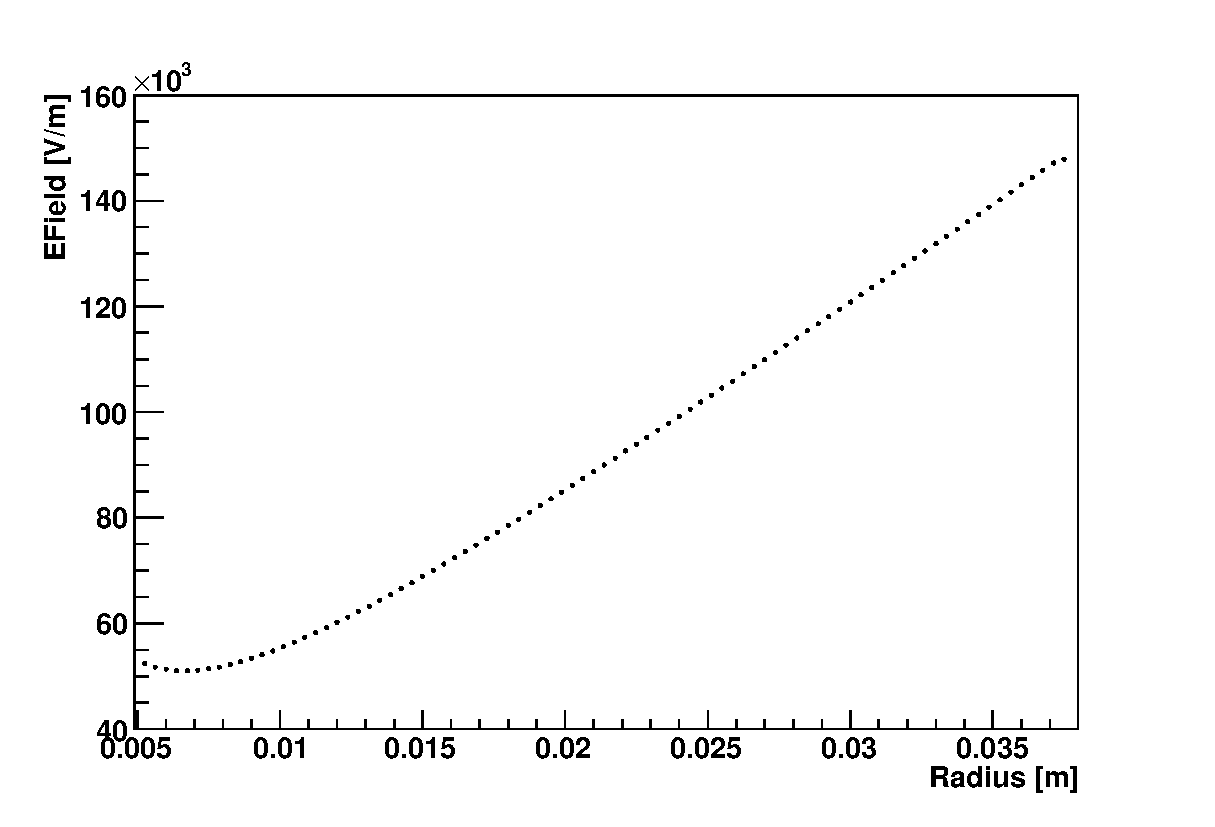
\includegraphics[width=0.49\textwidth]{EFieldNum.eps}
  \caption{Electric field as a function of radius r. (\emph{left}) Electric field from an analytical calculation according to \eqref{eq:EFieldAnalytical}. (\emph{right}) Electric field from a numerical calculation according to the method described in Sec.\,\ref{sec:field}. }
  \label{fig:efields}
\end{figure}
%%%%%%%%%%%%%%%

The relative difference of the electric field from the analytical and numerical calculation is shown in \figref{fig:efieldsRelDifference} as a function of the radius. The biggest deviation from the exact solution is of the order of $0.6$~\%.
%%%%%%%%
%%Figure: relative difference
%%%%%%%%
\begin{figure}[tbhp]
  \centering
  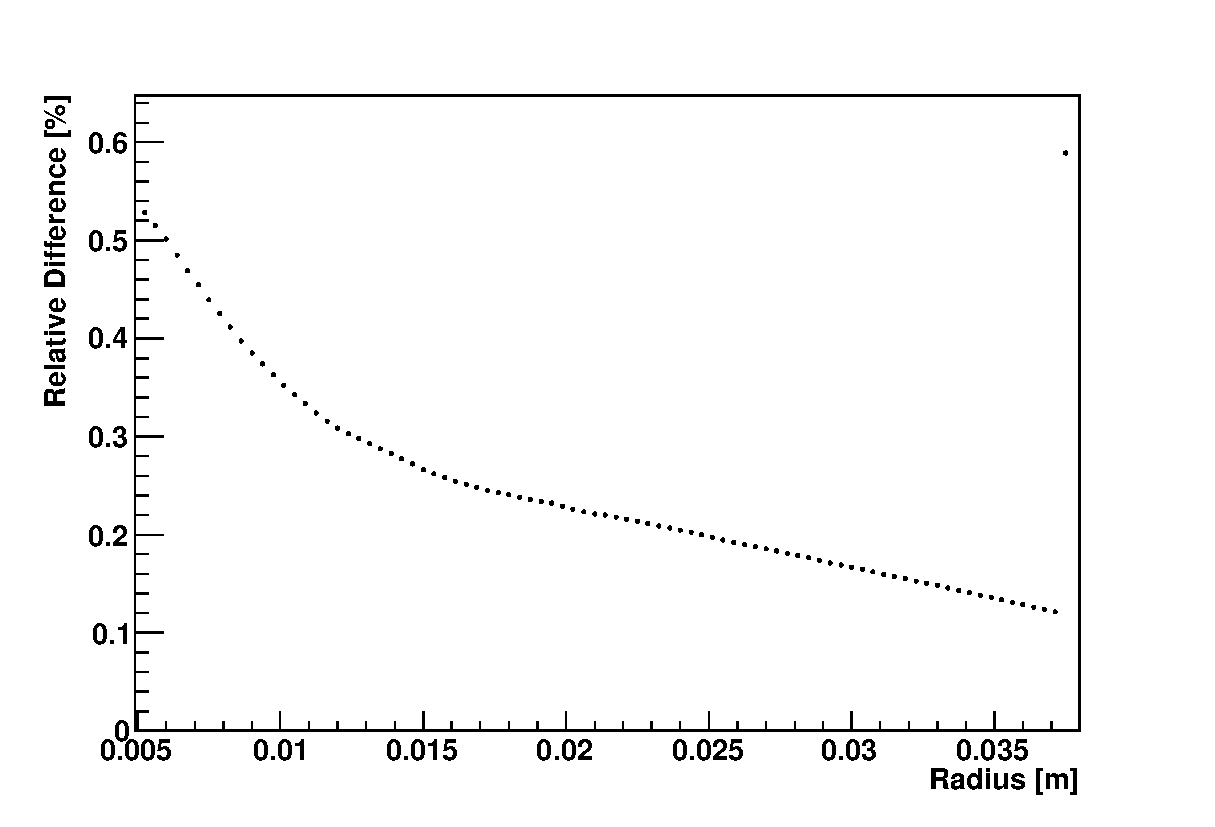
\includegraphics[width=0.8\textwidth]{relativeDifference_Num-Analyt.eps}
  \caption{Relative difference in \% in the electric fields from analytical to numerical calculation.}
  \label{fig:efieldsRelDifference}
\end{figure}
%%%%%%%%%%%%%%

%%% Local Variables:
%%% mode:latex
%%% TeX-master: "GSTR-08-M007"
%%% End:
